\chapter{Leçon 19: Transport, Gefierer a Vakanz}

\section{Transport an Ëmklammen / Transports et Correspondances / Transport and Transfers}

Besonnesch an enger Stad ass et wichteg, sech mam richtegen Transportmëttel auszedrécken. \textit{Surtout dans une ville, il est important de savoir s'exprimer avec le bon moyen de transport. / Especially in a city, it is important to express oneself using the correct means of transport.}

\subsection{Allgemeng Ausdréck / Expressions Générales / General Expressions}
\begin{itemize}
    \item \textbf{Ech komme vun niewendrun.} (Je viens d'à côté. / I come from next door.)
    \item \textbf{Ech hu mäi Bus verpasst.} (J'ai raté mon bus. / I missed my bus.)
    \item \textbf{Ech sinn zu Fouss komm.} (Je suis venu(e) à pied. / I came on foot.)
    \item \textbf{Ech huelen de Bus / den Zuch / den Tram.} (Je prends le bus / le train / le tram. / I take the bus / the train / the tram.)
    \item \textbf{Ech fuere mam Auto.} (Je conduis la voiture, j'y vais en voiture. / I drive, I go by car.)
\end{itemize}

\subsection{Eng Rees beschreiwen / Décrire un trajet / Describing a Journey}
Wann Dir musst erklären, wéi Dir op eng Plaz kommt, kënnt Dir folgend Sätz benotzen. \textit{Si vous devez expliquer comment vous arrivez à un endroit, vous pouvez utiliser les phrases suivantes. / If you need to explain how you get to a place, you can use the following sentences.}

\begin{itemize}
    \item \textbf{Ech komme vun Eech.} (Je viens d'Eich. / I come from Eich.)
    \item \textbf{Fir d'éischt huelen ech den Zuch bis a Pafendall...} (D'abord, je prends le train jusqu'à Pfaffenthal... / First, I take the train to Pfaffenthal...)
    \item \textbf{...an dann huelen ech den Tram fir op de Fluchhafen ze fueren.} (...et ensuite je prends le tram pour aller à l'aéroport. / ...and then I take the tram to go to the airport.)
    \item \textbf{Duerno klammen ech an de Bus ëm, fir heihin ze kommen.} (Ensuite, je change pour le bus pour arriver ici. / Then I change for the bus to get here.)
\end{itemize}

\vspace{1cm}

\section{Gefierer beschreiwen / Décrire une Voiture / Describing a Car}

Wéi beschreift een den eegenen Auto? \textit{Comment décrire sa propre voiture ? / How do you describe your own car?}

\begin{itemize}
    \item \textbf{Wat fir en Auto ass dat?} (Quelle sorte de voiture est-ce ? / What kind of car is that?)
    \item \textbf{Et ass en Elektroauto / en elektreschen Auto.} (C'est une voiture électrique. / It is an electric car.)
    \item \textbf{Et ass e Bensinsauto / en Dieselauto.} (C'est une voiture à essence / une voiture diesel. / It is a petrol car / a diesel car.)
    \item \textbf{Ech tanke kee Bensin, mäin Auto ass en Diesel.} (Je ne prends pas d'essence, ma voiture est un diesel. / I don't pump petrol, my car is a diesel.)
    \item \textbf{Wéi vill Päerd huet en?} (Combien de chevaux a-t-elle ? / How much horsepower does it have?)
    \item \textbf{Den Interieur ass aus Lieder. D'Sëtzer si ganz bequem.} (L'intérieur est en cuir. Les sièges sont très confortables. / The interior is leather. The seats are very comfortable.)
    \item \textbf{D'Steierrad läit gutt an der Hand.} (Le volant tient bien en main. / The steering wheel handles well.)
    \item \textbf{D'Spigele muss ee gutt astellen.} (Il faut bien régler les rétroviseurs. / You must adjust the mirrors well.)
    \item \textbf{Ech brauch nei Pneue fir de Wanter.} (J'ai besoin de nouveaux pneus pour l'hiver. / I need new tires for the winter.)
    \item \textbf{Den Auto huet e grousse Kofferraum.} (La voiture a un grand coffre. / The car has a large trunk.)
    \item \textbf{D'Faarf ass sëlwer.} (La couleur est argentée. / The color is silver.)
\end{itemize}

\vspace{1cm}

\section{De Wee op d'Aarbecht / Le Chemin du Travail / Commuting to Work}

\begin{itemize}
    \item \textbf{Wéi fuert dir op d'Aarbecht?} oder \textbf{Wéi gitt dir op d'Aarbecht?} (Comment allez-vous au travail ? / How do you go to work?)
    \item \textbf{Ech gi mam ëffentlechen Transport.} (Je vais en transports en commun. / I go by public transport.)
    \item \textbf{ëmklammen} (changer de moyen de transport, faire une correspondance / to change, to transfer).
    \item \textbf{Ech huelen de Bus bis op de Kierchbierg.} (Je prends le bus jusqu'au Kirchberg. / I take the bus up to Kirchberg.)
    \item \textbf{... bis op de Glacis.} (...jusqu'au Glacis. / ...up to the Glacis.)
    \item \textbf{... bis op d'Gare.} (...jusqu'à la gare. / ...up to the central station.)
\end{itemize}

\vspace{1cm}

\section{Vakanz an doriwwer eraus / Vacances et au-delà / Holidays and Beyond}

Mir schwätzen dacks iwwer eis Pläng fir d'Vakanz. \textit{Nous parlons souvent de nos projets pour les vacances. / We often talk about our holiday plans.}

\subsection{Sproochgebrauch fir d'Vakanz / Vacances / Holidays}
\begin{itemize}
    \item \textbf{Fir d'Vakanz: Et hänkt vun der Destinatioun of.} (Pour les vacances : Ça dépend de la destination. / For the holidays: It depends on the destination.)
    \item \textbf{Wann ech ausserhalb vun Europa reesen, huelen ech de Fliger.} (Quand je voyage en dehors de l'Europe, je prends l'avion. / When I travel outside of Europe, I take the plane.)
    \item \textbf{Zum Beispill vum Fluchhafe Lëtzebuerg bis op Frankfurt.} (Par exemple, de l'aéroport de Luxembourg jusqu'à Francfort. / For example, from Luxembourg airport to Frankfurt.)
    \item \textbf{Am August fuere mir a Griicheland fir mäi Cousin ze besichen.} (En août, nous partons en Grèce pour rendre visite à mon cousin. / In August, we go to Greece to visit my cousin.)
    \item \textbf{Ech ginn op Besuch.} (Je rends visite, je vais en visite. / I go for a visit.)
\end{itemize}

\subsection{Rees-Alternativen / Alternatives / Alternatives}
\begin{itemize}
    \item \textbf{Keng Vakanz, mir bleiwen hei.} (Pas de vacances, nous restons ici. / No holidays, we stay here.)
    \item \textbf{Ech reesen net gär, dofir ginn ech net an d'Vakanz.} (Je n'aime pas voyager, donc je ne pars pas en vacances. / I don't like to travel, therefore I don't go on holiday.)
    \item \textbf{D'Ouschtervakanz} (Les vacances de Pâques / Easter holidays).
    \item \textbf{E Fest} (Une fête / A festival or party).
\end{itemize}

\vspace{1cm}

\section{Kommissiounen / Faire les Courses / Grocery Shopping}

Och am Alldag brauche mir Transportmëttelen, fir kënnen anzekafen. \textit{Même au quotidien, nous avons besoin de moyens de transport pour pouvoir faire des achats. / Even in everyday life, we need transport to go shopping.}

\begin{itemize}
    \item \textbf{Wéi maacht dir är Kommissiounen?} (Comment faites-vous vos courses ? / How do you do your errands/groceries?)
    \item \textbf{akafen} (faire des achats / to go shopping).
    \item \textbf{Liewensmëttel kafen} (acheter de la nourriture, des provisions / to buy groceries, food).
    \item \textbf{Am Delhaize hei zu Lënster.} (Au Delhaize ici à Junglinster. / In the Delhaize here in Junglinster.)
    \item \textbf{An den Auchan goen.} (Aller à Auchan. / To go to Auchan.)
    \item \textbf{Alles ass nobäi.} (Tout est à proximité. / Everything is nearby.)
    \item \textbf{Ech ginn och meeschtens mam Auto akafen.} (Je vais aussi la plupart du temps faire les courses en voiture. / I also mostly go shopping by car.)
\end{itemize}

\vspace{1.5cm}
\color{geminiBlue}\hrule height 1.5pt \vspace{0.5em}\color{black}
\section{Vokabulär: Den Auto}

\begin{itemize}
    \item \textbf{e Pneu / e Rad} (Pl.: d'Pneuen / d'Rieder) $\rightarrow$ un pneu / une roue (a tire / a wheel)
    \item \textbf{e Spigel} (Pl.: d'Spigelen) $\rightarrow$ un rétroviseur (a mirror)
    \item \textbf{e Steierrad / e Volant} (Pl.: d'Steierrieder / d'Volanten) $\rightarrow$ un volant (a steering wheel)
    \item \textbf{e Sëtz} (Pl.: d'Sëtzer) $\rightarrow$ un siège (a seat)
\end{itemize}

\vspace{1em}

\begin{center}
    \begin{minipage}[t]{0.48\textwidth}
        \centering
        \framebox{\parbox{0.9\linewidth}{\centering
            \vspace{0.5cm}
            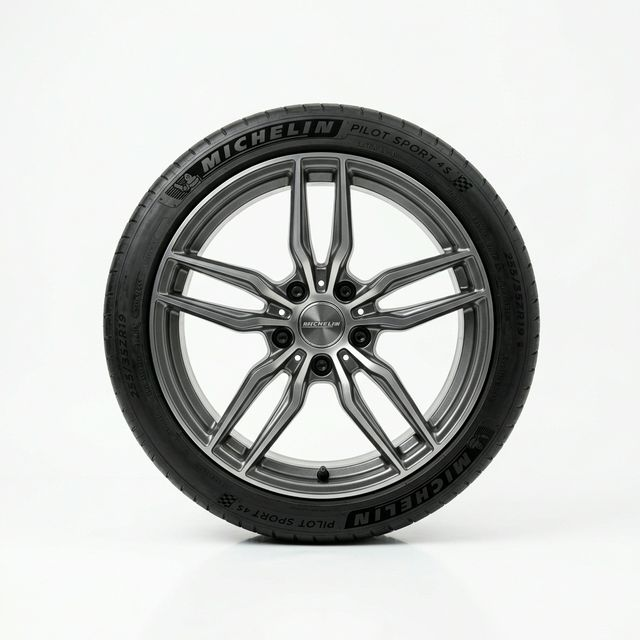
\includegraphics[width=0.9\linewidth]{vokab_300dpi/auto_rad.png} \\
            \small\textit{E Pneu / e Rad (Un pneu, une roue / A tire, a wheel)}
            \vspace{0.5cm}
        }}
    \end{minipage}
    \hfill
    \begin{minipage}[t]{0.48\textwidth}
        \centering
        \framebox{\parbox{0.9\linewidth}{\centering
            \vspace{0.5cm}
            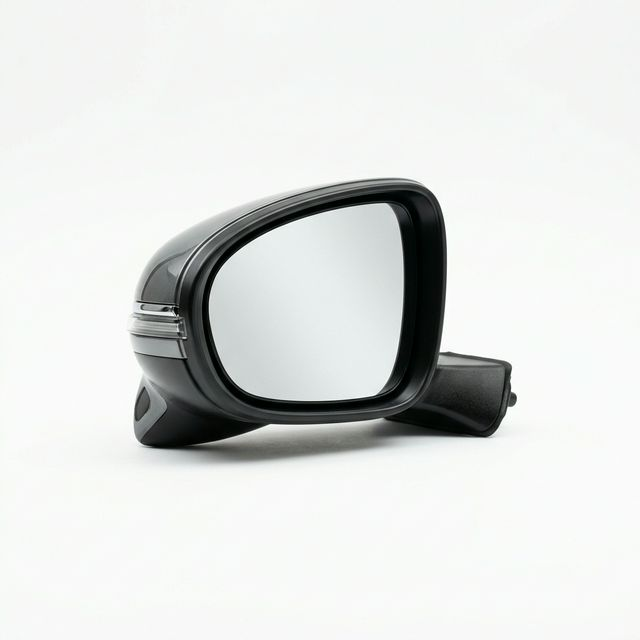
\includegraphics[width=0.9\linewidth]{vokab_300dpi/auto_spigel.png} \\
            \small\textit{E Spigel (Un rétroviseur / A mirror)}
            \vspace{0.5cm}
        }}
    \end{minipage}
    
    \vspace{1em}
    
    \begin{minipage}[t]{0.48\textwidth}
        \centering
        \framebox{\parbox{0.9\linewidth}{\centering
            \vspace{0.5cm}
            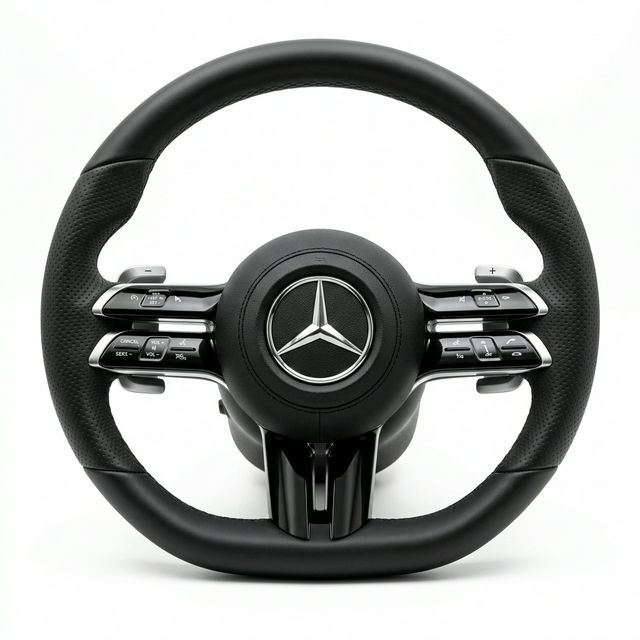
\includegraphics[width=0.9\linewidth]{vokab_300dpi/auto_steierrad.png} \\
            \small\textit{E Steierrad / e Volant (Un volant / A steering wheel)}
            \vspace{0.5cm}
        }}
    \end{minipage}
    \hfill
    \begin{minipage}[t]{0.48\textwidth}
        \centering
        \framebox{\parbox{0.9\linewidth}{\centering
            \vspace{0.5cm}
            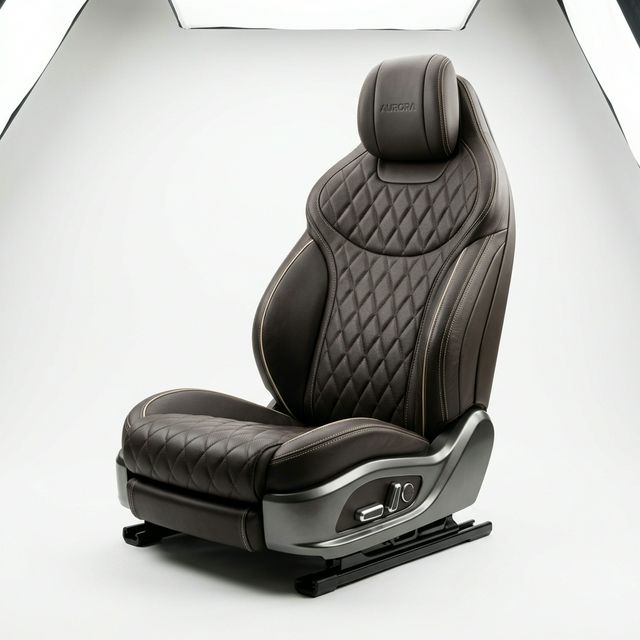
\includegraphics[width=0.9\linewidth]{vokab_300dpi/auto_setz.png} \\
            \small\textit{E Sëtz (Un siège / A seat)}
            \vspace{0.5cm}
        }}
    \end{minipage}
\end{center}
